\documentclass{jsreport}
\usepackage[dvipdfmx]{graphicx}
\usepackage{comment}
\title{方式設計仕様書}
% 方式設計仕様書 (ファイル名:system_design_spec.pdf) 「どのように実現するか」  

\begin{comment}
    方式設計では, 設計する計算機に対する要求仕様を定め, それを実現するための技\\
術的裏付けを求める.

    方式設計レベルの仕様書は, それさえあれば誰がその先の設計を行っても, システ\\
ムの機能, 性能が同一となるように記述されている必要がある. したがって本実験の場\\
合には, 完成した計算機があるプログラムを実行した場合に その実行サイクル数が一致\
することが求められよう.

    具体的には, 提出する方式設計仕様書には 設計する計算機に関する以下の項目が含\
まれる:

        概要, 目的, 目標, 設計方針, 特長.
        命令セット・アーキテクチャ (SIMPLE アーキテクチャ からの変更点).
        構造 (structure) と動作 (behavior). それらを説明するための以下の図表:
 ブロック図
            フェーズ・フロー・チャート
            データ・フロー・チャート
        (SIMPLE 設計資料 の SIMPLE/B からの変更点).
        高速化/並列処理の方式. それらを説明するためのブロック図, フェーズ・フローチャート, データ・フローチャート.
        性能/コストの予測. その実現可能性, 妥当性.

    なお, 配布資料に書いてあるようなことを再掲する必要はない. 必要であれば, 参考文献として挙げ, 適宜引用すること.

    SIMPLE 設計資料における SIMPLE/B の記述は, 方式設計レベルの仕様書である.
\end{comment}

\author{グループ番号:20 \\ 学生番号1029285143 原口卓也\\ 学生番号1029287621 宮城竜大}
\date{\today}
\begin{document}

\maketitle
\clearpage

\section{概要}
        SIMPLEアーキテクチャをベースとし、いくつかの拡張をもって改良したものを作成する。\\
       具体的には、命令セットの拡張(ADDI、SUBI、BR、BALの追加)とパイプライン化を行う。

\section{命令セット・アーキテクチャ (SIMPLE アーキテクチャ からの変更点)}
        \subsection{即値演算命令の追加}
                演算/入出力命令に即値演算命令を追加\\
        即値演算命令:レジスタRdとdの加算または減算の結果をRdに格納し、条件コードを設定する。条件コードCには最上位ビットからの桁上げが設定される

    \subsection{Branch Register, Branch And Link命令の追加}
                即値ロード/無条件分岐命令にBranch Register、Branch And Link命令を追加\\
        Branch And Link:関数を呼び出した命令の次のPCをレジスタに格納し、関数の先頭にジャンプする\\
        Branch Register:レジスタに格納された値をPCに書き込む

    \subsection{パイプライン化}
        p1/p2/p3/p4/p5の並列実行を可能にしパイプライン化する。

\section{構造 (structure) と動作 (behavior)}
図\ref{fig:block}は現在完成しているプロセッサのブロック図である。
パイプライン化すると、各フェーズ間にレジスタが挟まるが、流れるデータ自体は変わらないので、そのまま流用することとした。

\begin{figure}[h]
\centering
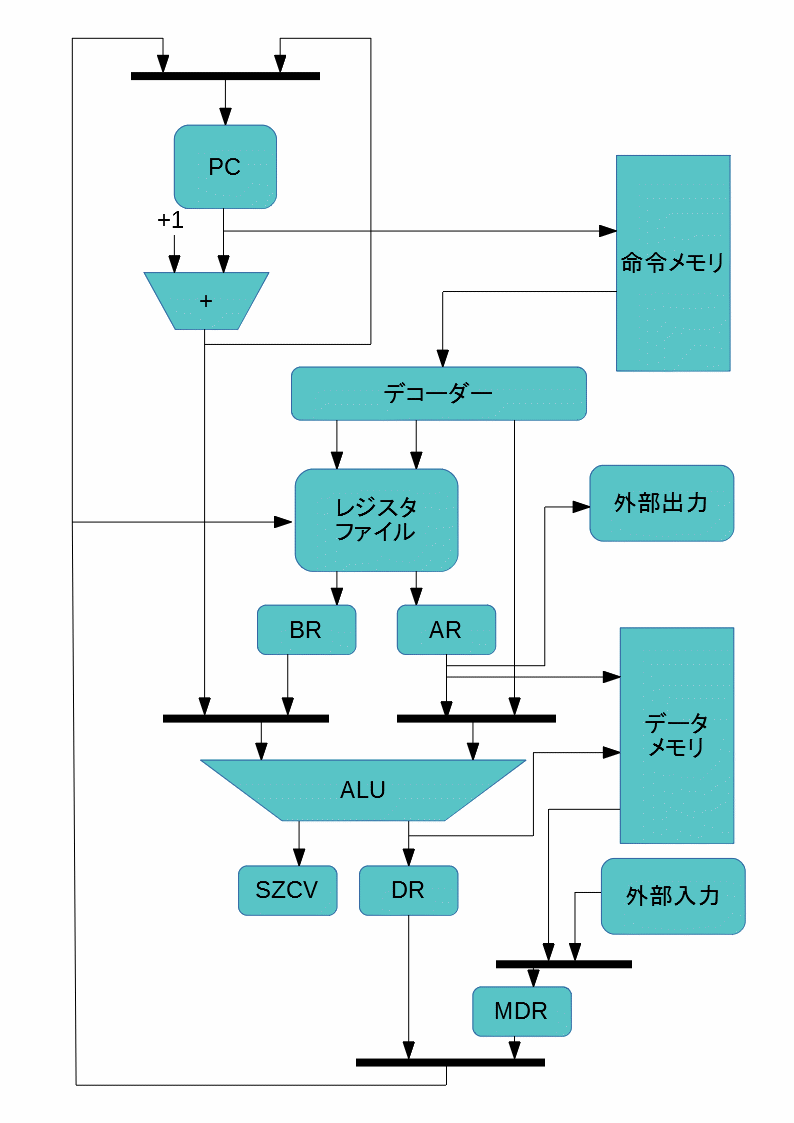
\includegraphics[width=120mm]{figures/data_flow.png}
\caption{ブロック図}
\label{fig:block}
\end{figure}

図\ref{fig:phase}は今回製作するプロセッサのフェーズフローである。

\begin{figure}[h]
\centering
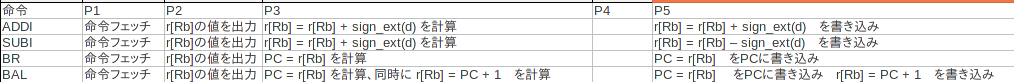
\includegraphics[width=180mm]{figures/phase.png}
\caption{フェーズフロー}
\label{fig:phase}
\end{figure}

\begin{figure}[h]
\centering
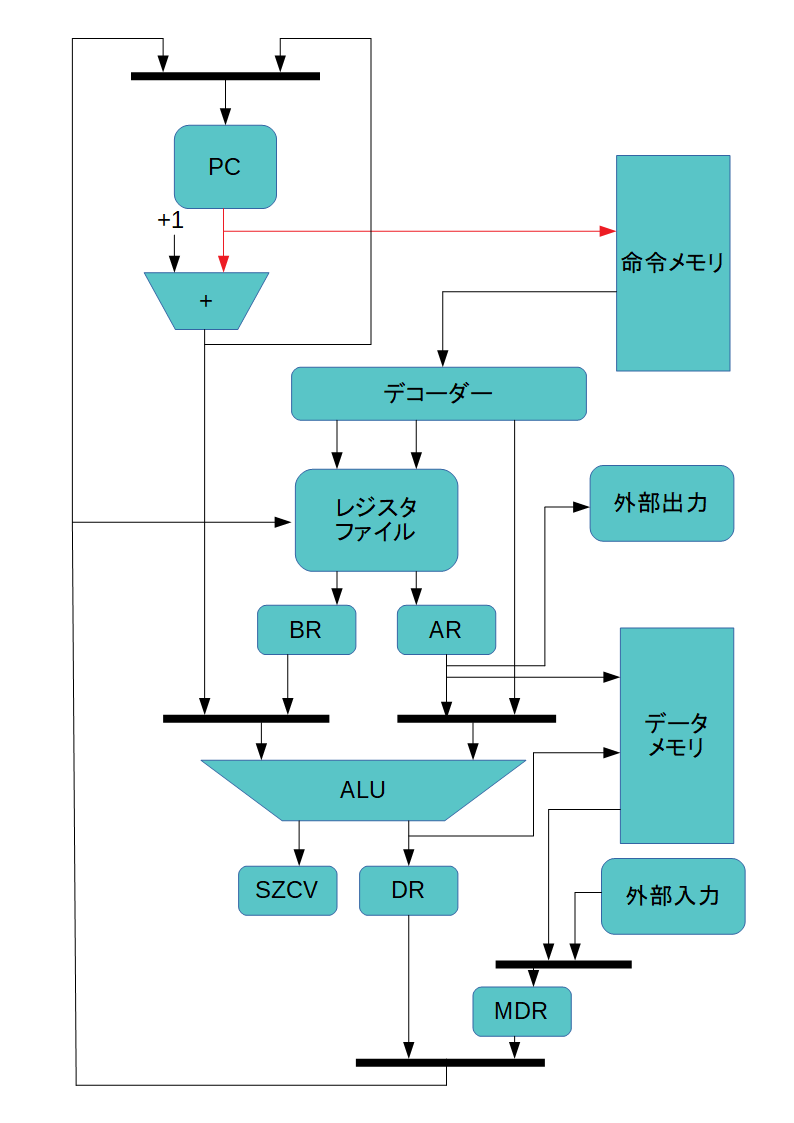
\includegraphics[width=60mm]{figures/phase1.png}
\caption{phase1}
\label{fig:phase1}
\end{figure}
\begin{figure}[h]
\centering
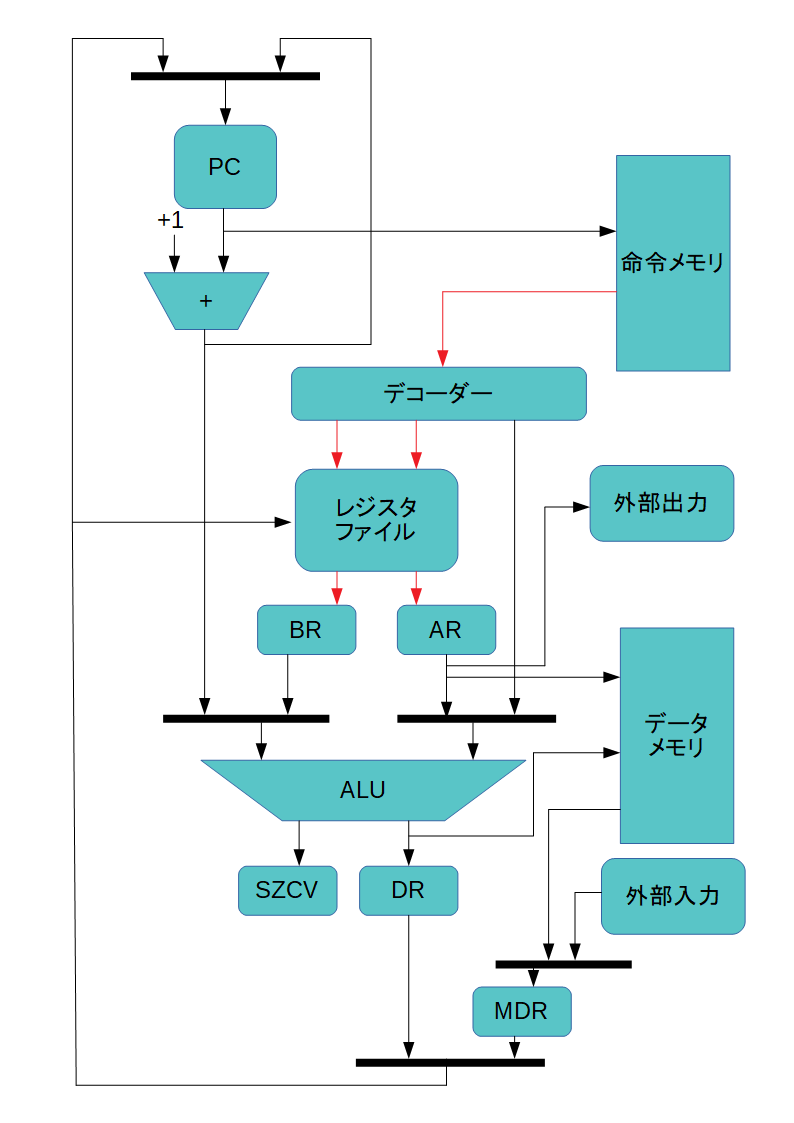
\includegraphics[width=60mm]{figures/phase2.png}
\caption{phase2}
\label{fig:phase2}
\end{figure}
\begin{figure}[h]
\centering
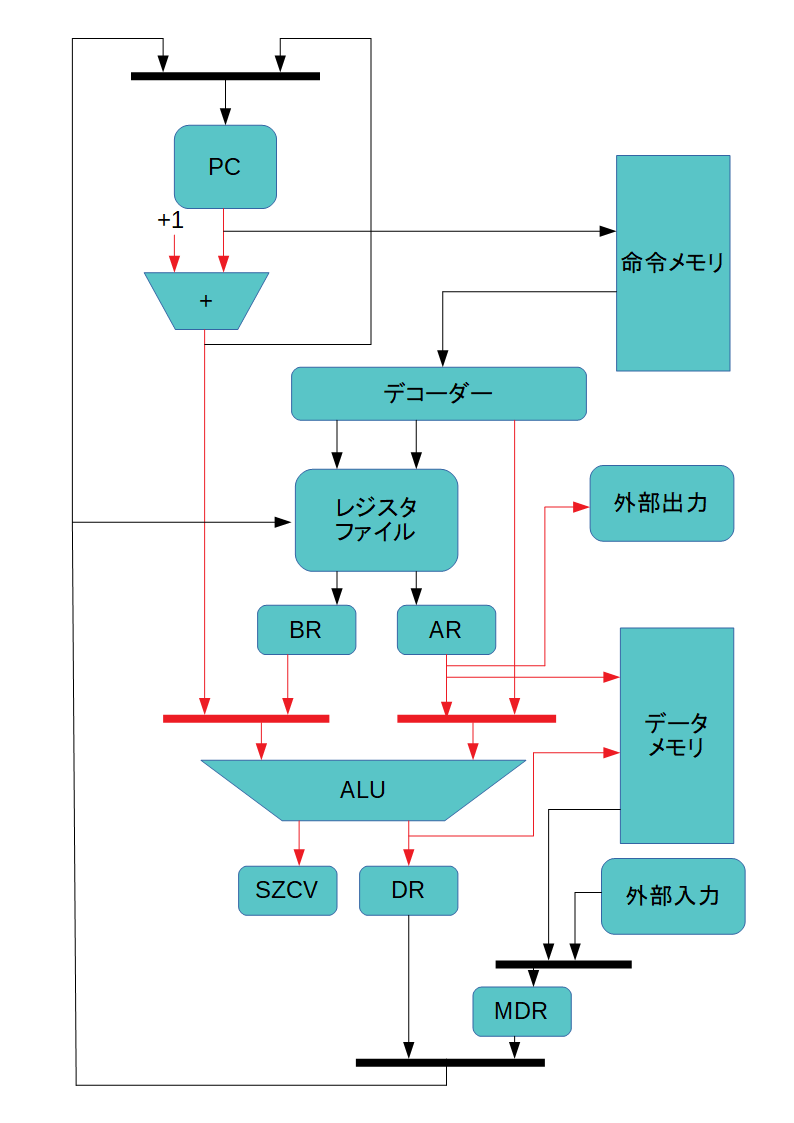
\includegraphics[width=60mm]{figures/phase3.png}
\caption{phase3}
\label{fig:phase3}
\end{figure}
\begin{figure}[h]
\centering
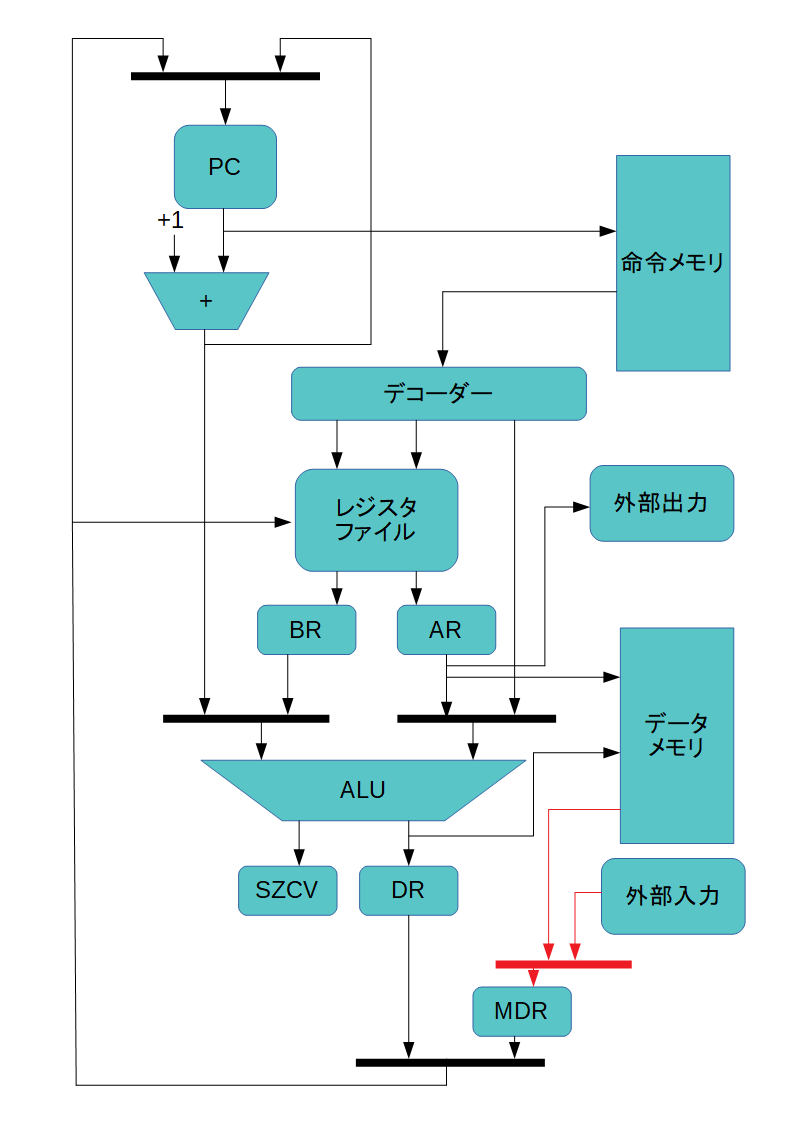
\includegraphics[width=60mm]{figures/phase4.png}
\caption{phase4}
\label{fig:phase4}
\end{figure}
\begin{figure}[h]
\centering
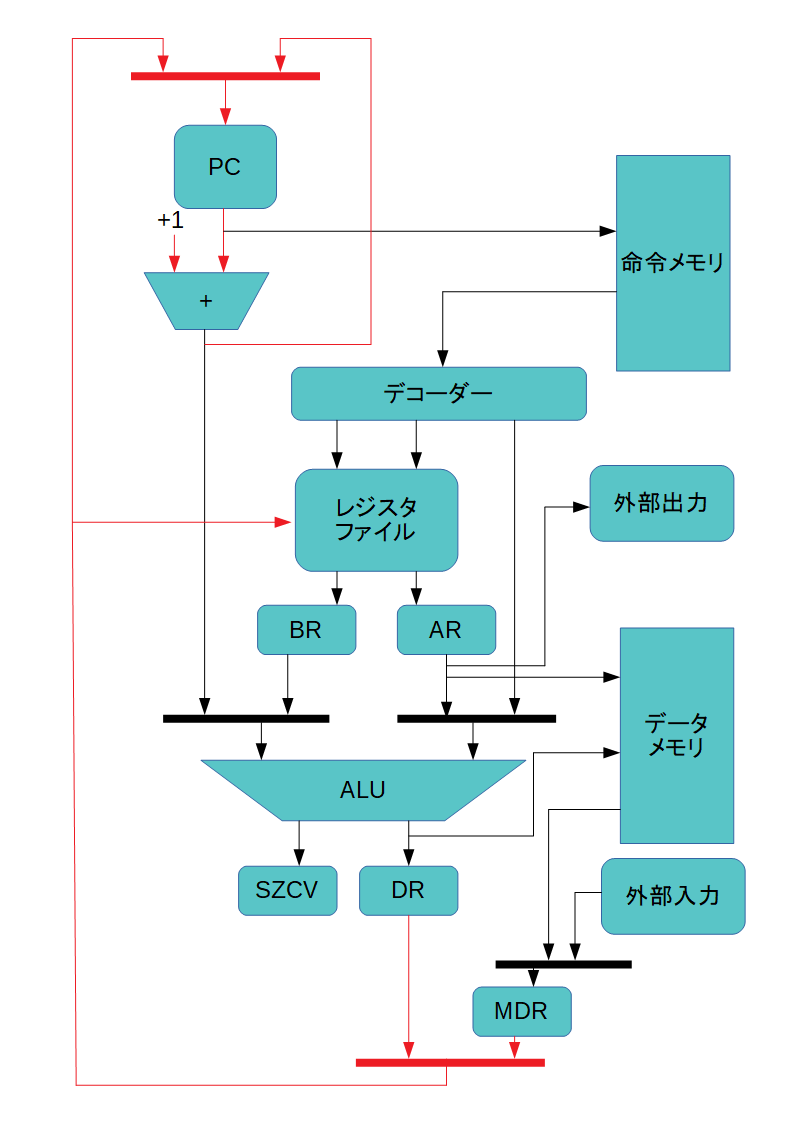
\includegraphics[width=60mm]{figures/phase5.png}
\caption{phase5}
\label{fig:phase5}
\end{figure}

%%%%%%%%%%%%%%%%%%%%%%%%%%%%%%%%%%%%%%%%%%%%%%%%%%%%%%%%%%%%%%%%%%%%%%%%                                                                                                                                                              
% todo                                                                                                                                                                                                                                
%%%%%%%%%%%%%%%%%%%%%%%%%%%%%%%%%%%%%%%%%%%%%%%%%%%%%%%%%%%%%%%%%%%%%%%%                                                                                                                                                              

\end{document}


